% Author: Rasmus Pank Roulund
\documentclass{standalone}
\usepackage{tikz}
\usetikzlibrary{shapes.geometric,automata,arrows,positioning,patterns,calc,fit,intersections}
\usepackage{standalone}

\usepackage{pgfplots}
\usepackage{relsize}
\usepackage{amssymb}


 
\begin{document}

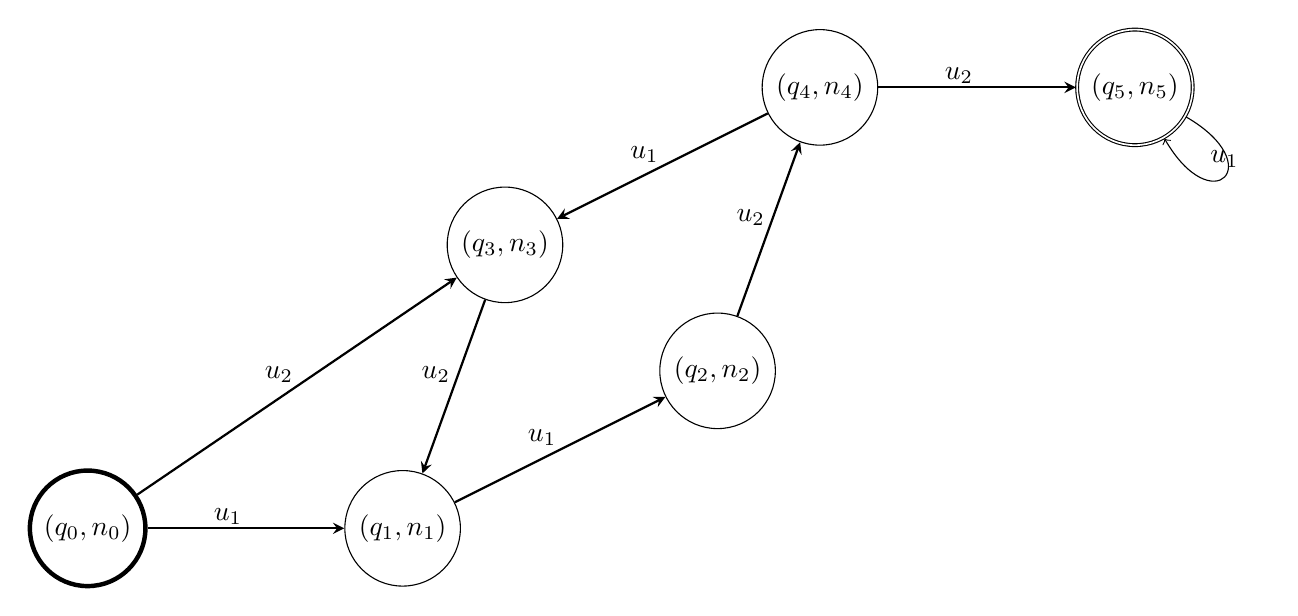
\begin{tikzpicture}[node distance = 4cm]

\tikzstyle{cell} = [circle,draw]
\tikzstyle{cont} = [thick,->,>=stealth]
\tikzstyle{labels} = [anchor=south east,inner sep=1pt]

%% ------------------
%% -- OFFLINE PART --
%% ------------------

 \newcommand*\nodeonecolor{}
 \newcommand*\nodetwocolor{}
 \newcommand*\nodethreecolor{}
 \newcommand*\nodefourcolor{}
 \newcommand*\nodefivecolor{}
 \newcommand*\nodesixcolor{}
 \only<+->{}
 \only<+->{\renewcommand*\nodeonecolor{red}}
 \only<+->{\renewcommand*\nodetwocolor{red}}
 \only<+->{\renewcommand*\nodethreecolor{red}}
 \only<+->{\renewcommand*\nodefivecolor{red}}
 \only<+->{\renewcommand*\nodesixcolor{red}}

\node (init) [cell,line width=1.6pt,\nodeonecolor] {$(q_0,n_0)$};
\node (n1) [cell,right of = init,\nodetwocolor] {$(q_1,n_1)$};
\node (n2) [cell,right of = n1,yshift = 2cm,\nodethreecolor] {$(q_2,n_2)$};
\node (n3) [cell,left of = n2,yshift = 1.6cm,xshift=1.3cm,\nodefourcolor] {$(q_3,n_3)$};
\node (n4) [cell,right of = n3,yshift=2cm,\nodefivecolor] {$(q_4,n_4)$};
\node (g) [cell,accepting, right of = n4,\nodesixcolor] {$(q_5,n_5)$};


\draw[cont,\nodetwocolor] (init) -- node[labels] {$u_1$} (n1);
\draw[cont] (init) -- node[labels] {$u_2$} (n3);
\draw[cont,\nodethreecolor] (n1) -- node[labels] {$u_1$} (n2);
\draw[cont] (n3) -- node[labels] {$u_2$} (n1);
\draw[cont,\nodefivecolor] (n2) -- node[labels] {$u_2$} (n4);
\draw[cont] (n4) -- node[labels] {$u_1$} (n3);
\draw[cont,\nodesixcolor] (n4) -- node[labels] {$u_2$} (g);
\path (g) edge [->,out=330,in=300,looseness=8,\nodesixcolor] node[above] {$u_1$} (g);
\end{tikzpicture}

\end{document}